\chapter{微分几何}

\newenvironment{slamcase}[1]{%
    \par\noindent\textbf{\color{main}例：#1}\rmfamily\par
}{%
    \par\ignorespacesafterend
}

本章把第三章的拓扑流形继续推进到可微流形，并把这条数学主线接到SLAM中的状态估计。核心问题不是把流形看成一张弯曲的图，而是说明：为什么在不同局部坐标之间切换后，速度、导数、Jacobian和优化方向仍然代表同一个几何对象。

本章遵循如下顺序：
\[
\begin{aligned}
&\text{拓扑流形}
\longrightarrow \text{可微结构}
\longrightarrow \text{可微映射与微分同胚}
\longrightarrow \text{切空间} \\
&\longrightarrow \text{向量场、推前与拉回}
\longrightarrow \text{向量空间、对偶与张量}
\longrightarrow \text{度量、长度与能量}.
\end{aligned}
\]
其中，切空间提供局部线性化空间，推前给出观测Jacobian的几何来源，拉回解释梯度为何由$J^\top r$产生，而度量负责把协向量表示成梯度向量。第五章将在此基础上进一步说明李群$\SE(3)$如何通过指数映射实现合法的位姿更新。

%——————————————————————————————————%

\section{从拓扑流形到可微流形}

\subsection{拓扑流形还缺少什么}

第三章中的拓扑流形只要求每个点附近看起来像某个欧氏空间。更正式地，Hausdorff、第二可数的拓扑空间$M$若满足：对每个$p\in M$，都存在开邻域$U\subset M$和$\mathbb R^n$中开集$W$，使得$U$与$W$同胚，则称$M$为$n$维拓扑流形。

这个定义足以讨论开集、邻域、连续曲线、连通性和紧性，但还不足以讨论速度和导数。把地球表面$S^2$想成一个空间：拓扑结构可以告诉我们哪些区域是邻域、两条路径是否连续、两个区域是否连通；可是如果没有额外规则，我们还不能保证不同地图上计算出的速度是同一个几何量。

设粒子轨迹为$\gamma(t)\in M$。在地图$x$中，它的坐标轨迹是
\[
    t\longmapsto x(\gamma(t))\in\mathbb R^n.
\]
如果换到另一张地图$y$，则
\[
    y(\gamma(t))
    =(y\circ x^{-1})(x(\gamma(t))).
\]
因此，速度是否存在、速度如何变换，取决于坐标转换$y\circ x^{-1}$是否可微；加速度则还需要坐标转换具有二阶可微性。可微结构的真正作用，就是规定哪些局部坐标之间的转换是允许的，从而使微积分不依赖于地图的选择。

\begin{slamcase}{拓扑结构与可微结构的分工}
拓扑结构回答“点附近是什么样的”和“连续变化是否成立”；可微结构进一步回答“局部变化率是什么”。在SLAM中，前者支撑状态空间的局部性和连续性，后者支撑位姿扰动、观测模型微分、Jacobian以及局部优化。
\end{slamcase}

\subsection{$C^k$结构与光滑结构}

这里的$C^k$表示连续可微$k$阶：函数本身以及直到$k$阶的偏导数都连续。一个$C^1$结构足以让我们讨论速度和切向量，$C^2$结构允许进一步讨论加速度以及部分曲率概念，而$C^\infty$结构允许任意阶的光滑微分几何运算。

从拓扑流形到可微流形的层次可以写成
\[
\begin{array}{c}
\text{集合 }M\\[-2pt]
\downarrow\ \text{赋予拓扑}\\[-2pt]
\text{拓扑空间 }(M,\mathcal O)\\[-2pt]
\downarrow\ \text{局部欧氏、Hausdorff、第二可数}\\[-2pt]
\text{拓扑流形}\\[-2pt]
\downarrow\ \text{加入兼容的 }C^k\text{ 图册}\\[-2pt]
\text{$C^k$ 可微流形}\\[-2pt]
\downarrow\ k=\infty\\[-2pt]
\text{光滑流形}.
\end{array}
\]

\begin{definition}[可微结构]
设$M$是$n$维拓扑流形。若一族坐标图两两满足$C^k$兼容性，并且覆盖$M$，则称其为一个$C^k$图册。包含所有与该图册兼容的坐标图的极大$C^k$图册称为一个$C^k$可微结构。
\end{definition}

带有一个$C^k$可微结构的拓扑流形称为$C^k$可微流形；当$k=\infty$时，通常简称为光滑流形。后文主要讨论光滑流形，因此“可微”默认指$C^\infty$，除非明确写出有限的$k$。

\begin{remark}[关于有限阶可微结构]
在许多常见的有限维流形中，有限阶可微结构可以与光滑结构建立联系，但精确的平滑化结论涉及更深入的理论和维数条件。本笔记只需要光滑流形来定义切空间、推前、拉回和李群，因此不把“任意$C^k$结构都无条件包含$C^\infty$结构”作为基础结论。
\end{remark}

%——————————————————————————————————%

\section{图、图册与坐标转换}

\subsection{图与坐标函数}

设$M$是$n$维拓扑流形。

\begin{definition}[图]
一张图（chart）是二元组$(U,x)$，其中$U\subset M$是开集，且
\[
    x:U\to x(U)\subset\mathbb R^n
\]
是同胚。这里$x$是坐标映射，$x(p)$是点$p$在这张局部地图中的坐标，并且$x(U)$必须是$\mathbb R^n$中的开集。
\end{definition}

图中的三个对象不能混淆：$U$是流形上的局部区域，$x$是把该区域画到欧氏空间的映射，而$x(p)$只是点$p$在这套坐标下的坐标值。图并不是说$M$整体等于$\mathbb R^n$，而是说$M$的这一小块可以用$n$个实数局部描述。

\begin{definition}[图册]
一族图$\mathcal A=\{(U_\alpha,x_\alpha)\}$若满足
\[
    M=\bigcup_\alpha U_\alpha,
\]
则称为$M$的一个图册（atlas）。
\end{definition}

球面不能用一张没有奇点的平面地图覆盖，但可以用多张局部地图覆盖。这正是图册的必要性：每张图只负责一个局部区域，不要求任何单张坐标图是全局参数化。

\subsection{坐标转换}

设$(U,x)$和$(V,y)$是两张相交的图，且$U\cap V\neq\varnothing$。同一个点$p\in U\cap V$有两套坐标$x(p)$和$y(p)$。从$x$坐标转换到$y$坐标的映射是
\[
    y\circ x^{-1}:
    x(U\cap V)\to y(U\cap V).
\]
它的逆映射是
\[
    x\circ y^{-1}:y(U\cap V)\to x(U\cap V).
\]
对任意$p\in U\cap V$，有
\[
    x(p)\xrightarrow{\ y\circ x^{-1}\ }y(p).
\]
其中$x^{-1}$先把$x$坐标还原成流形上的同一个点，$y$再把该点写成另一套坐标。

\begin{center}
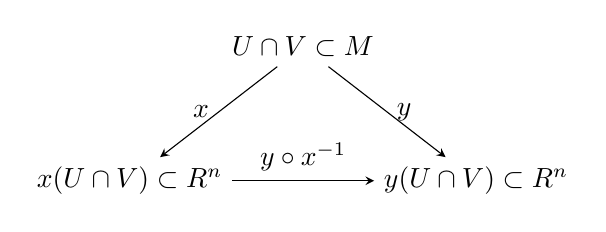
\begin{tikzpicture}[>=stealth]
    \node (M) at (0,1.7) {$U\cap V\subset M$};
    \node (X) at (-2.2,0) {$x(U\cap V)\subset\mathbb R^n$};
    \node (Y) at (2.2,0) {$y(U\cap V)\subset\mathbb R^n$};
    \draw[->] (M) -- node[left] {$x$} (X);
    \draw[->] (M) -- node[right] {$y$} (Y);
    \draw[->] (X) -- node[above] {$y\circ x^{-1}$} (Y);
\end{tikzpicture}
\end{center}

\begin{definition}[$C^k$兼容]
两张图$(U,x)$和$(V,y)$称为$C^k$兼容，如果$U\cap V=\varnothing$，或坐标转换
\[
    y\circ x^{-1}:x(U\cap V)\to y(U\cap V)
\]
及其逆
\[
    x\circ y^{-1}:y(U\cap V)\to x(U\cap V)
\]
都是$C^k$映射。
\end{definition}

必须同时要求正向与反向转换都是$C^k$。只有这样，沿一条曲线计算出的速度和加速度才不会因为换图而失去可微性。

\begin{definition}[$C^k$图册与极大图册]
一个覆盖$M$且任意两张图都$C^k$兼容的图册称为$C^k$图册。若一张新图与图册中的所有图都$C^k$兼容，则把它加入图册并不会改变可微规则。包含所有这类兼容图的图册称为极大$C^k$图册。
\end{definition}

极大图册不是“随意挑选最多的图”，而是把同一种坐标微积分规则下所有允许的局部地图都收集起来。一个$C^k$可微流形可以写为$(M,\mathcal O,\mathcal A)$，分别表示底层集合、拓扑和极大$C^k$图册。

\subsection{立方根坐标：为什么兼容性不可省略}

\begin{slamcase}{立方根坐标}
令$M=\mathbb R$，考虑两张图
\[
    (\mathbb R,\operatorname{id}),
    \qquad
    (\mathbb R,\chi),
    \qquad
    \chi(a)=a^{1/3}.
\]
因为$\chi$是同胚，所以两张图作为拓扑图都合法。它们的坐标转换为
\[
    \chi\circ\operatorname{id}^{-1}(a)=a^{1/3},
    \qquad
    \operatorname{id}\circ\chi^{-1}(u)=u^3.
\]
反向变换$u\mapsto u^3$光滑，但正向变换在$0$处不可微，因为
\[
    \frac{d}{da}a^{1/3}=\frac{1}{3a^{2/3}}
\]
在$a=0$处没有有限值。因此这两张图不是$C^1$兼容的。

考虑曲线$\gamma(t)=t$。标准坐标下
\[
    \frac{d}{dt}\operatorname{id}(\gamma(t))=1;
\]
而在$\chi$坐标下
\[
    \frac{d}{dt}\chi(\gamma(t))=\frac{d}{dt}t^{1/3}
\]
在$t=0$处不存在有限导数。这个例子说明的不是实数线本身变得奇怪，而是同一个拓扑空间上的两套局部坐标可能对“什么叫可微”给出不兼容的判断。$C^1$兼容性正是为了排除这种坐标依赖。
\end{slamcase}

\subsection{从流形到李群}

在可微流形上再加入一个群结构，并要求群乘法与求逆都是光滑映射，就得到李群。层次关系为
\[
\text{集合}
\to\text{拓扑空间}
\to\text{拓扑流形}
\to\text{可微流形}
\to\text{李群}.
\]
第五章中的$\SO(3)$与$\SE(3)$同时具有群结构和光滑流形结构，因此可以使用本章的切空间、微分和局部线性化，也可以使用李群的指数映射进行合法位姿更新。

%——————————————————————————————————%

\section{可微映射与微分同胚}

\subsection{流形映射的局部表达}

设$M$、$N$分别为$m$维、$n$维光滑流形，$\varphi:M\to N$为映射，$p\in M$。取$M$上的图$(U,x)$和$N$上的图$(V,y)$，满足$p\in U$、$\varphi(p)\in V$，并在需要时缩小$U$使$\varphi(U)\subset V$。则$\varphi$在这些局部坐标下的表达为
\[
    y\circ\varphi\circ x^{-1}:
    x(U)\subset\mathbb R^m\to y(V)\subset\mathbb R^n.
\]

\begin{center}
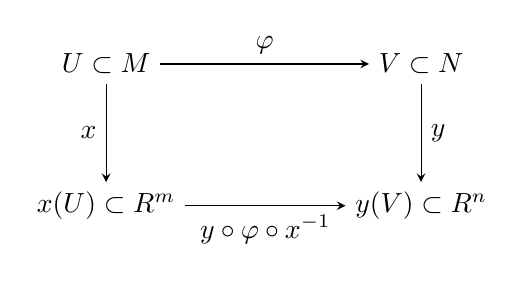
\begin{tikzpicture}[>=stealth]
    \node (M) at (0,1.8) {$U\subset M$};
    \node (N) at (4,1.8) {$V\subset N$};
    \node (MX) at (0,0) {$x(U)\subset\mathbb R^m$};
    \node (NY) at (4,0) {$y(V)\subset\mathbb R^n$};
    \draw[->] (M) -- node[above] {$\varphi$} (N);
    \draw[->] (M) -- node[left] {$x$} (MX);
    \draw[->] (N) -- node[right] {$y$} (NY);
    \draw[->] (MX) -- node[below] {$y\circ\varphi\circ x^{-1}$} (NY);
\end{tikzpicture}
\end{center}

\begin{definition}[$C^k$映射]
映射$\varphi:M\to N$称为在$p$处$C^k$，如果上述局部坐标表达$y\circ\varphi\circ x^{-1}$在$x(p)$处是$C^k$的。若对所有$p\in M$都成立，则称$\varphi$为$C^k$映射；$C^\infty$映射称为光滑映射。
\end{definition}

这个定义与坐标选择无关。若改用图$(U',x')$与$(V',y')$，新的坐标表达可以写成
\[
    y'\circ\varphi\circ(x')^{-1}
    =
    (y'\circ y^{-1})
    \circ(y\circ\varphi\circ x^{-1})
    \circ(x\circ(x')^{-1}).
\]
两侧的坐标转换都是$C^k$，中间映射也是$C^k$，所以由复合的稳定性得到相同的可微性结论。

\begin{theorem}[光滑复合与链式法则]
若$\varphi:M\to N$和$\psi:N\to P$光滑，则$\psi\circ\varphi$光滑。它们的微分满足
\[
    d(\psi\circ\varphi)_p
    =d\psi_{\varphi(p)}\circ d\varphi_p.
\]
\end{theorem}

\begin{slamcase}{SLAM中的观测映射}
位姿、地图点和相机内参组成状态与参数，投影模型把它们映射到像素观测。例如在$Z_C>0$的区域，针孔投影
\[
    \pi(X_C,Y_C,Z_C)
    =
    \begin{bmatrix}
        f_xX_C/Z_C+c_x\\
        f_yY_C/Z_C+c_y
    \end{bmatrix}
\]
是光滑映射。SLAM能够在当前估计附近计算观测Jacobian，前提正是相关状态落在投影定义域内，并且整体观测模型在该处光滑。
\end{slamcase}

\subsection{微分同胚}

\begin{definition}[微分同胚]
若光滑映射$\varphi:M\to N$是双射，且逆映射$\varphi^{-1}:N\to M$也光滑，则称$\varphi$为微分同胚，记作
\[
    M\cong_{\mathrm{diff}}N.
\]
\end{definition}

集合双射只保留元素之间的一一对应；同胚还保留连续性、邻域和连通性；微分同胚进一步保留可微性、切向量和微分。微分同胚的两个流形可视为同一个可微空间的不同表示。

\begin{slamcase}{不同坐标表示的同一可微空间}
一张合法坐标图$(U,x)$与另一张$C^\infty$兼容坐标图$(U,y)$并不是两个不同的物理空间，而是同一局部流形的两种坐标表示。SLAM代码中使用的增量坐标、李代数坐标或其他局部参数化，也应被理解为同一状态流形上的局部表示，而不是把状态流形永久替换成一个全局欧氏空间。
\end{slamcase}

\subsection{可微结构的唯一性问题}

拓扑结构与光滑结构并不总是唯一对应。低维情形通常较为刚性，但从四维开始可能出现同一个拓扑流形带有不同光滑结构的深刻现象；最著名的例子是存在不可数多个彼此不微分同胚的exotic $\mathbb R^4$。不同维数下光滑结构的存在、数量和分类是微分拓扑中的高阶问题，与本笔记后续的SLAM推导无关，因此这里只保留这个提醒，不使用未经条件限定的维数分类结论。

%——————————————————————————————————%

\section{切空间：局部速度的空间}

拓扑流形的局部欧氏性告诉我们“附近像$\mathbb R^n$”，可微结构则使我们能够比较曲线的一阶变化。切空间$T_pM$由所有经过$p$的光滑曲线在$p$处可能产生的瞬时速度组成，是流形在点$p$处的局部线性化空间。

\subsection{坐标曲线与瞬时速度}

设$(U,x)$是包含$p$的坐标图，写$x=(x^1,\ldots,x^n)$。在坐标域中，经过$x(p)$的第$a$条坐标曲线为
\[
    \alpha_a(t)=x(p)+t e_a,
\]
其中$e_a$是$\mathbb R^n$的第$a$个标准基向量。将它拉回流形，得到
\[
    \gamma_a(t)=x^{-1}(\alpha_a(t)),
    \qquad
    \gamma_a(0)=p.
\]
这条曲线只沿第$a$个坐标方向变化。

\begin{figure}[htbp]
    \centering
    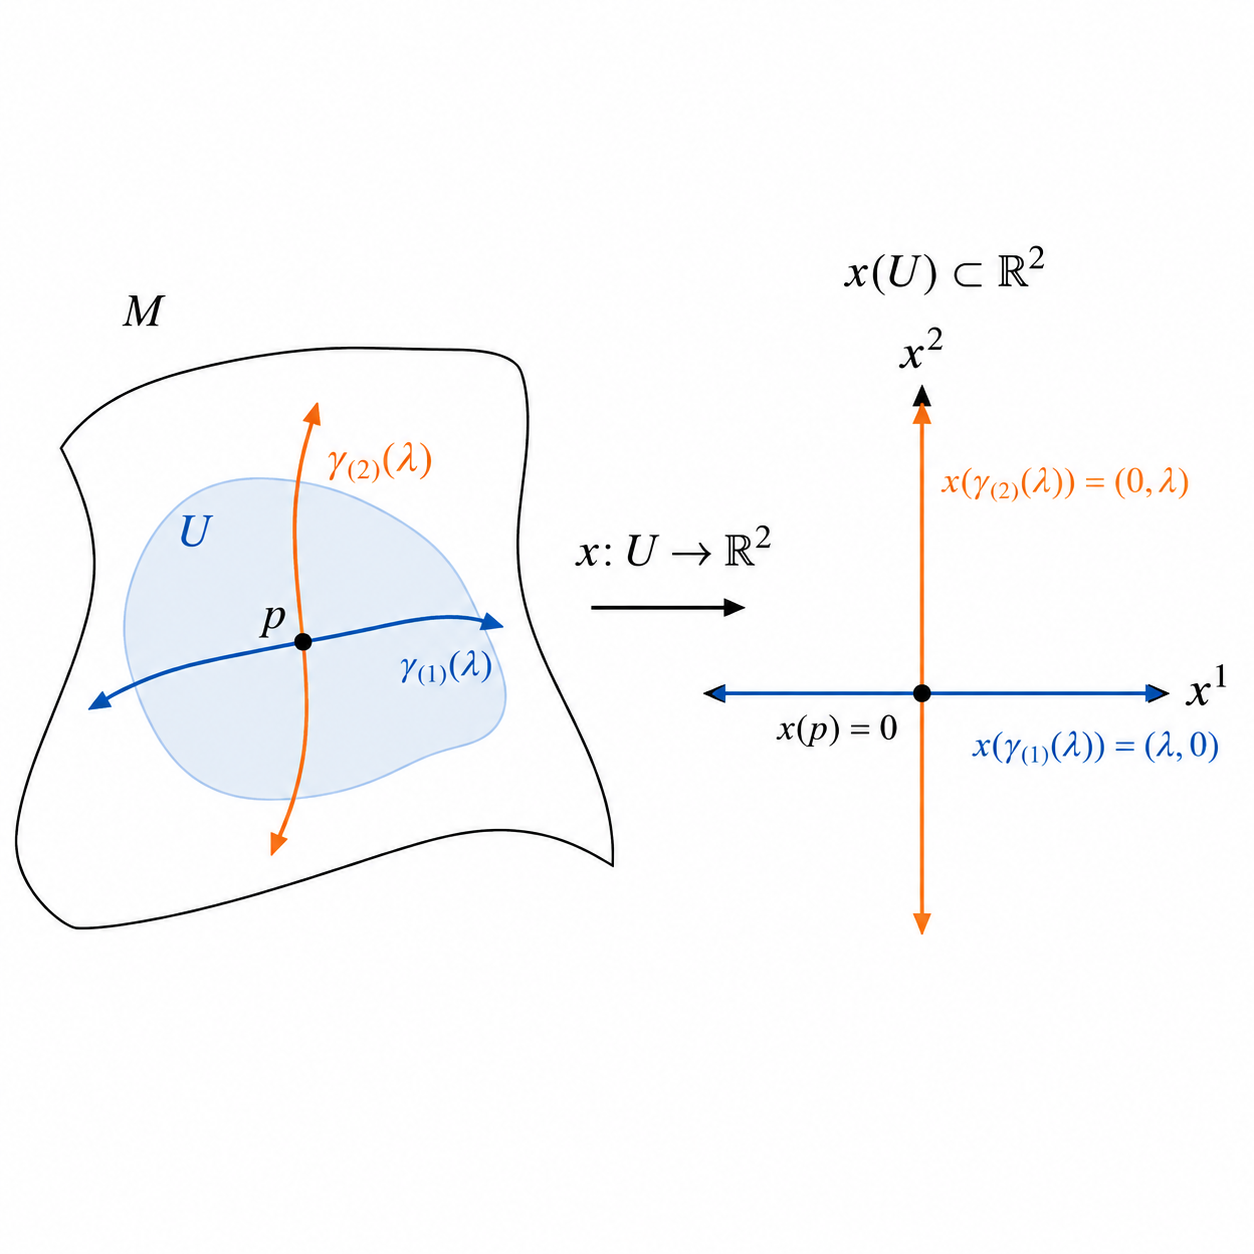
\includegraphics[width=0.78\textwidth]{assets/images/chapter4/4_2/1782550067546-a8df09f72cfb.png}
    \caption{坐标图把流形中的局部曲线转换为欧氏坐标中的曲线。}
    \label{fig:chapter4-chart-curves}
\end{figure}

\begin{definition}[曲线诱导的切向量]
设$\gamma:(-\varepsilon,\varepsilon)\to M$是光滑曲线，且$\gamma(0)=p$。若两条曲线$\gamma_1,\gamma_2$在$p$处满足：对一个、等价地对任意包含$p$的坐标图$(U,x)$，都有
\[
    \left.\frac{d}{dt}\right|_{0}x(\gamma_1(t))
    =
    \left.\frac{d}{dt}\right|_{0}x(\gamma_2(t)),
\]
则称它们在$p$处一阶等价。等价类记为$[\gamma]_p$，由所有等价类组成的向量空间记为$T_pM$，称为$p$处的切空间。
\end{definition}

可微兼容性保证了“一阶等价”与坐标选择无关。曲线本身不是切向量；切向量只记录曲线经过$p$时的一阶变化信息。

\subsection{切向量作为导子}

\begin{definition}[导子]
点$p\in M$处的一个导子是线性映射$X:C^\infty(M)\to\mathbb R$，满足Leibniz法则
\[
    X(fg)=f(p)X(g)+g(p)X(f),
    \qquad f,g\in C^\infty(M).
\]
\end{definition}

\begin{theorem}[曲线速度与导子等价]
曲线$\gamma$在$p=\gamma(0)$处诱导的切向量对光滑函数$f$的作用定义为
\[
    X_{\gamma,p}[f]
    :=\left.\frac{d}{dt}\right|_{0}f(\gamma(t)).
\]
它是一个导子；反过来，每个$p$处的导子都由某条经过$p$的光滑曲线的速度唯一确定。因此，切向量既可以理解为曲线的瞬时速度，也可以理解为作用在函数上的方向导数。
\end{theorem}

在局部坐标$(U,x)$下，定义坐标基向量
\[
    \left(\frac{\partial}{\partial x^a}\right)_p[f]
    :=
    \left.
    \frac{\partial(f\circ x^{-1})}{\partial u^a}
    \right|_{u=x(p)}.
\]
若$\gamma$的坐标曲线为$\alpha(t)=x(\gamma(t))$，则由多元链式法则
\[
    X_{\gamma,p}
    =
    \sum_{a=1}^{n}
    \left.\frac{d\alpha^a}{dt}\right|_{0}
    \left(\frac{\partial}{\partial x^a}\right)_p.
\]

\begin{theorem}[切空间的坐标基]
对$n$维光滑流形$M$和$p\in M$，坐标基
\[
    \left\{
    \left(\frac{\partial}{\partial x^1}\right)_p,ldots,
    \left(\frac{\partial}{\partial x^n}\right)_p
    \right\}
\]
构成$T_pM$的一组基。因此
\[
    \dim T_pM=n.
\]
\end{theorem}

这个结论是“$n$维流形在无穷小尺度上像$\mathbb R^n$”的精确表达。切空间是线性空间，但整个流形通常不是线性空间。

\begin{figure}[htbp]
    \centering
    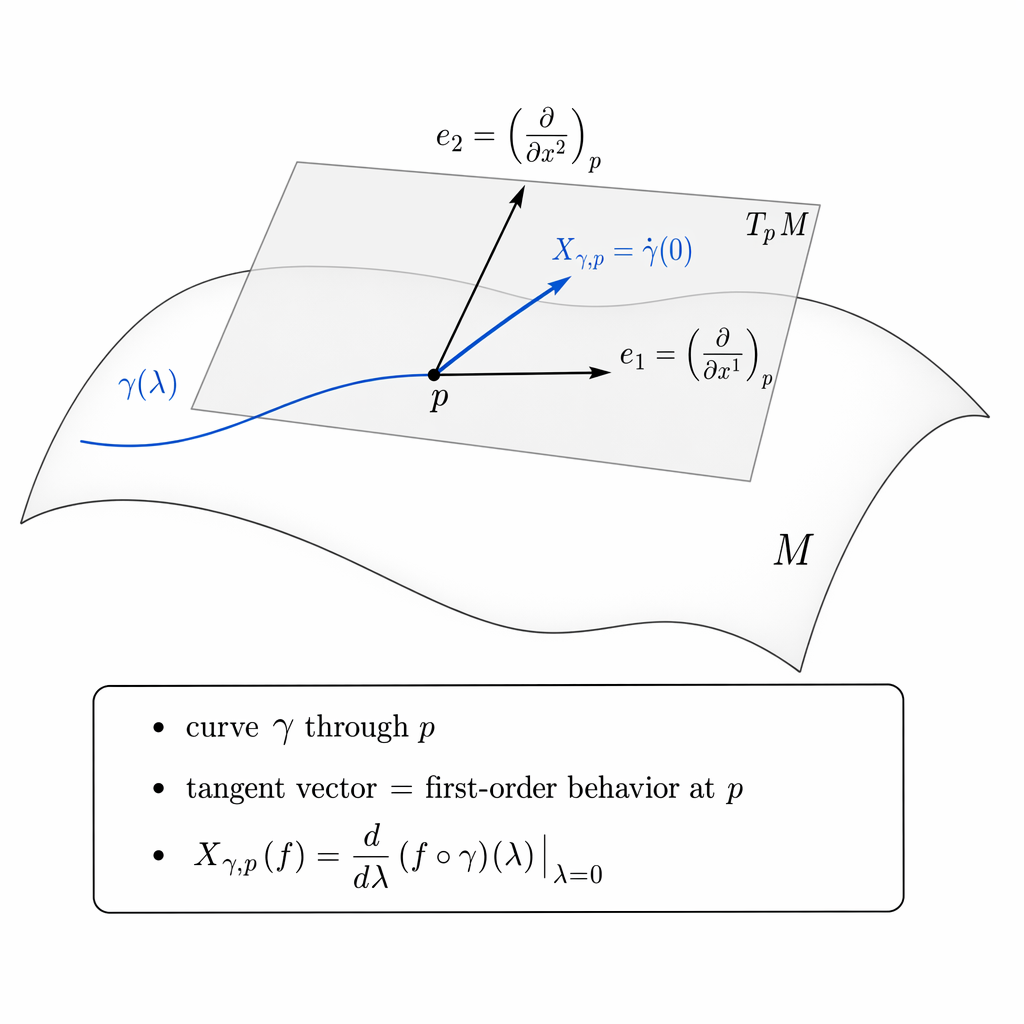
\includegraphics[width=0.78\textwidth]{assets/images/chapter4/4_2/dim_tan_vector.png}
    \caption{切向量是经过$p$的曲线在$p$处的一阶速度，坐标基张成$T_pM$。}
    \label{fig:chapter4-tangent-basis}
\end{figure}

\subsection{球面的切平面}

\begin{slamcase}{球面上的合法瞬时速度}
把$S^2$嵌入$\mathbb R^3$，取$p\in S^2$。若$\gamma(t)\in S^2$且$\gamma(0)=p$，则
\[
    \gamma(t)^\top\gamma(t)=1.
\]
对$t$求导并在$0$处取值，得到
\[
    p^\top\dot\gamma(0)=0.
\]
因此
\[
    T_pS^2
    =\{v\in\mathbb R^3:p^\top v=0\}.
\]
粒子可以沿球面的任意切向方向瞬时运动，却不能把法向方向作为球面上的合法瞬时速度。这个例子体现了约束状态空间的基本特征。
\end{slamcase}

\subsection{$\SE(3)$的切空间与局部扰动}

三维位姿空间可表示为
\[
    \SE(3)=
    \left\{
    \begin{bmatrix}R&t\\0&1\end{bmatrix}
    :R\in\SO(3),\ t\in\mathbb R^3
    \right\}.
\]
若
\[
    T(t)=
    \begin{bmatrix}R(t)&t(t)\\0&1\end{bmatrix}
\]
是一条经过$T$的光滑曲线，则
\[
    \dot R(0)=R\Omega,
    \qquad \Omega^\top=-\Omega,
    \qquad \dot t(0)\in\mathbb R^3.
\]
因此
\[
    T_T\SE(3)
    =
    \left\{
    \begin{bmatrix}R\Omega&v\\0&0\end{bmatrix}
    :\Omega^\top=-\Omega,\ v\in\mathbb R^3
    \right\},
    \qquad
    \dim T_T\SE(3)=3+3=6.
\]
这里的六维只是切空间的维数；它不意味着$\SE(3)$整体就是$\mathbb R^6$。

在当前点$p$附近，如果选定局部坐标或retraction，可以把切向量写成$\xi\in\mathbb R^n$，并记局部更新为
\[
    p_{\mathrm{new}}=p\boxplus\xi.
\]
符号$\boxplus$强调这不是普通加法，而是“用切空间增量生成流形上的新点”。对$\SE(3)$，第五章会用李群指数映射把它具体写成$T_{\mathrm{new}}=T\Exp(\delta\xi^\wedge)$。

\begin{figure}[htbp]
    \centering
    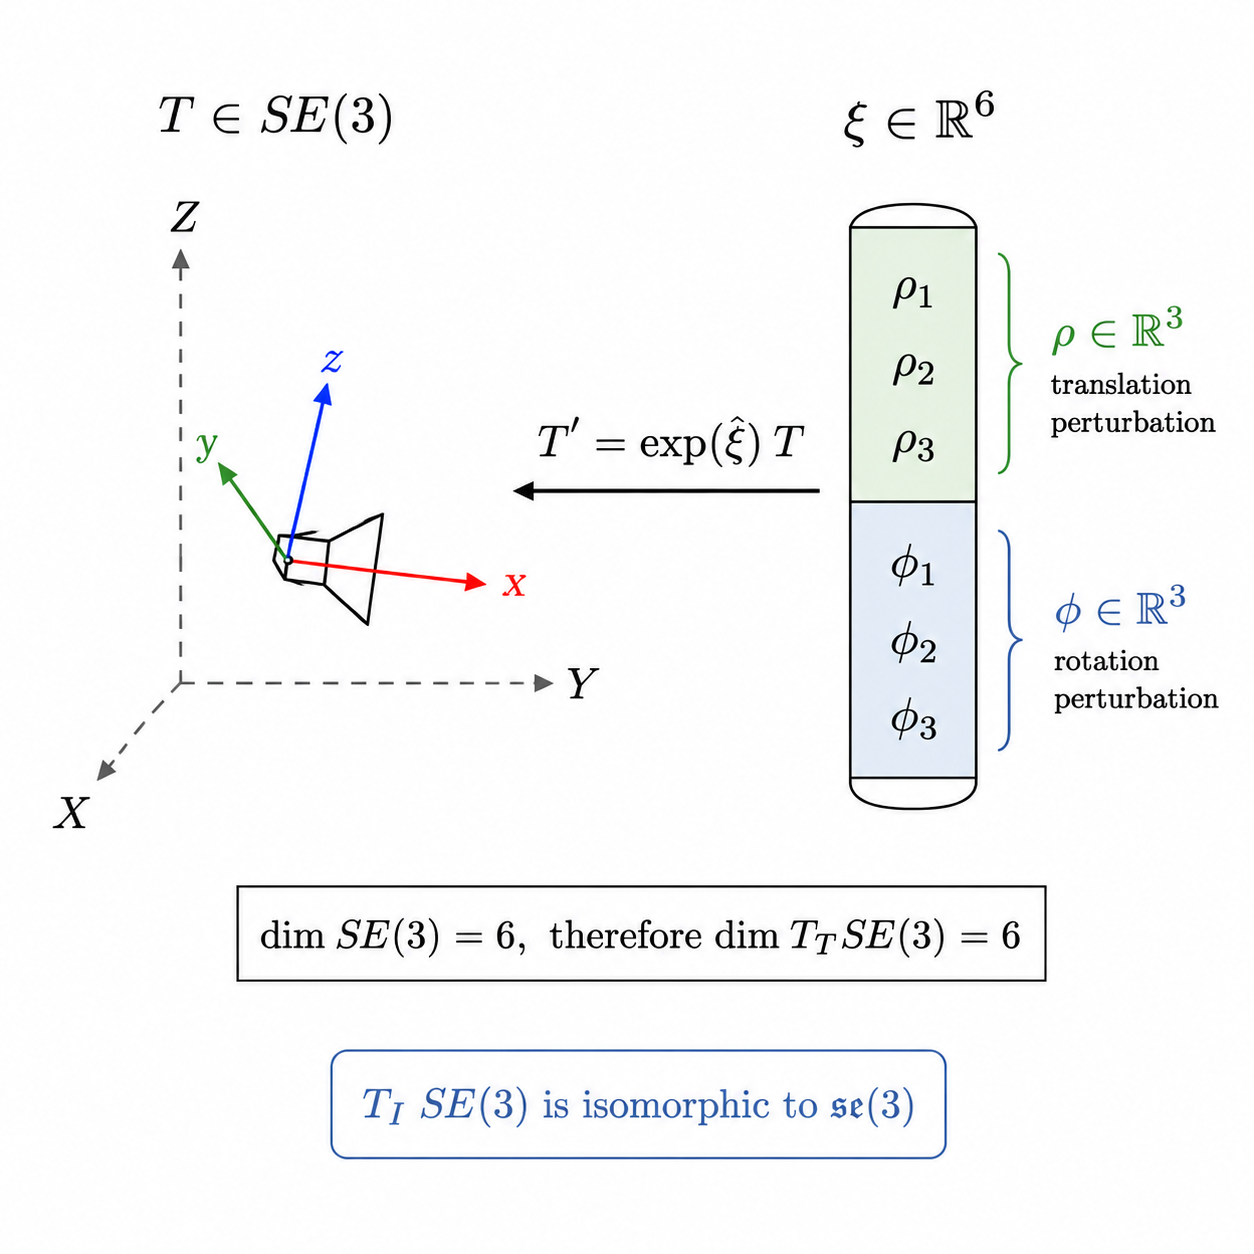
\includegraphics[width=0.78\textwidth]{assets/images/chapter4/4_2/1782550365901-c8c107252aa5.png}
    \caption{$\SE(3)$的位姿局部扰动由三维平移和三维旋转共同组成。}
    \label{fig:chapter4-se3-tangent}
\end{figure}

\subsection{切空间的几个边界}

\begin{enumerate}
    \item 曲线是定义域为区间的映射，切向量是曲线在某点处的一阶等价类，二者不能混为一谈。
    \item $T_pM$是线性空间，而$M$一般不是线性空间。只有在选定局部图、retraction或李群指数映射后，才可以把局部增量写成坐标向量。
    \item 切空间依赖于基点。$T_pM$和$T_qM$通常是不同的向量空间，不能在没有额外结构时直接相加；李群的左平移将在第五章中提供一种自然的搬运方式。
    \item $dF_p$属于余切空间$T_p^\ast M$，而梯度属于切空间$T_pM$。二者的联系需要度量，不能仅凭记号把它们视为同一个对象。
\end{enumerate}

%——————————————————————————————————%

\section{向量场、推前与拉回}

前面是在一个点$p$处讨论局部速度。若要描述整个状态空间中的运动，就需要在每个点指定一个切向量，这得到向量场；若要把局部运动送入观测空间，就需要推前；若要把观测空间中的测量规则带回状态空间，就需要拉回。

\subsection{向量场与积分曲线}

\begin{definition}[向量场]
流形$M$上的向量场是在每个点$p\in M$指定一个切向量
\[
    X_p\in T_pM
\]
的规则，记为$X:p\mapsto X_p$。若它在任意局部坐标下的分量函数都光滑，则称$X$为光滑向量场。
\end{definition}

在坐标$(x^1,\ldots,x^n)$下，光滑向量场写为
\[
    X_p=\sum_{a=1}^{n}X^a(p)
    \left(\frac{\partial}{\partial x^a}\right)_p.
\]
这里$X^a$是随点变化的函数，不是一个在整个流形上固定不变的向量。

\begin{definition}[积分曲线]
若光滑曲线$\gamma:I\to M$满足
\[
    \dot\gamma(t)=X_{\gamma(t)},
    \qquad \gamma(0)=p,
\]
则称$\gamma$为向量场$X$从$p$出发的积分曲线。
\end{definition}

这个方程是坐标无关的内蕴微分方程：左侧是曲线在流形上的瞬时速度，右侧是向量场在当前位置指定的速度。选定坐标后，它才变成关于坐标分量的普通微分方程。

\begin{slamcase}{向量场与SLAM状态运动}
设机器人状态空间为流形$\mathcal M$。连续运动模型可以抽象为
\[
    X_x\in T_x\mathcal M,
    \qquad x\in\mathcal M,
\]
状态轨迹满足$\dot x(t)=X_{x(t)}$。第五章将把这个思想用于李群：给定单位元处的局部运动方向$\xi\in T_eG$，通过左平移构造
\[
    X_g^\xi=(dL_g)_e\xi,
\]
再由积分曲线定义指数映射。这样“当前状态处的允许速度”不需要被误认为是一个固定的全局欧氏向量。
\end{slamcase}

\subsection{推前：局部速度如何穿过映射}

\begin{definition}[推前]
设$\varphi:M\to N$为光滑映射，$p\in M$。$\varphi$在$p$处的推前（也记为微分）是线性映射
\[
    d\varphi_p=\varphi_{\ast,p}:T_pM\to T_{\varphi(p)}N.
\]
若把切向量视为导子，则对$X\in T_pM$，$d\varphi_pX$由
\[
    (d\varphi_pX)(f)=X(f\circ\varphi),
    \qquad f\in C^\infty(N)
\]
唯一确定。
\end{definition}

如果$X$由曲线$\gamma(0)=p$诱导，则由链式法则
\[
    d\varphi_p(X_{\gamma,p})
    =X_{\varphi\circ\gamma,\,\varphi(p)}
    =\left.\frac{d}{dt}\right|_{0}(\varphi\circ\gamma)(t).
\]
因此，推前把输入流形中的一阶运动送到输出流形中的一阶运动；它不是把两个流形的点直接相减。

\begin{center}
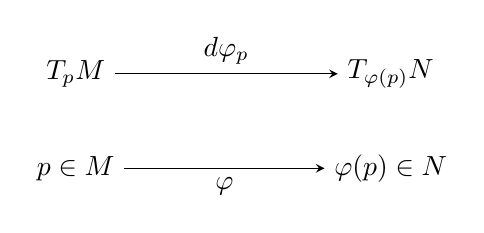
\begin{tikzpicture}[>=stealth]
    \node (Tp) at (0,0) {$T_pM$};
    \node (Tq) at (4,0) {$T_{\varphi(p)}N$};
    \node (p) at (0,-1.2) {$p\in M$};
    \node (q) at (4,-1.2) {$\varphi(p)\in N$};
    \draw[->] (Tp) -- node[above] {$d\varphi_p$} (Tq);
    \draw[->] (p) -- node[below] {$\varphi$} (q);
\end{tikzpicture}
\end{center}

\subsection{残差、观测模型与Jacobian}

\begin{definition}[残差函数]
设状态空间为流形$\mathcal M$，观测空间为$\mathcal Z$，观测模型为光滑映射
\[
    h:\mathcal M\to\mathcal Z.
\]
给定真实测量$z$。当观测空间是欧氏空间，或已经选定了观测空间的局部坐标时，定义
\[
    r(x)=z-h(x)\in\mathbb R^m.
\]
残差是向量值函数，记录当前状态预测与真实测量之间尚未解释的向量差。
\end{definition}

\begin{definition}[加权最小二乘代价]
给定多个残差$r_i:\mathcal M\to\mathbb R^{m_i}$及权重矩阵$W_i$，定义
\[
    F(x)=\frac12\sum_i r_i(x)^\top W_i r_i(x).
\]
若第$i$个观测噪声协方差为可逆矩阵$\Sigma_i$，通常取$W_i=\Sigma_i^{-1}$。
\end{definition}

残差是向量值函数，代价是待最小化的标量函数。文献中“error”有时指残差，有时指残差平方和或代价，必须根据上下文区分这两个层次。

\begin{slamcase}{单目视觉SLAM的重投影残差}
设相机位姿为
\[
    T_{CW}=(R,t)\in\SE(3),
    \qquad R\in\SO(3),\quad t\in\mathbb R^3,
\]
地图点为$P_W\in\mathbb R^3$。从世界坐标变换到相机坐标：
\[
    P_C=RP_W+t
    =\begin{bmatrix}X_C&Y_C&Z_C\end{bmatrix}^{\top},
    \qquad Z_C>0.
\]
针孔模型为
\[
    \pi(P_C)=
    \begin{bmatrix}
        f_xX_C/Z_C+c_x\\
        f_yY_C/Z_C+c_y
    \end{bmatrix}.
\]
若实际像素为$z\in\mathbb R^2$，则
\[
    r(T_{CW},P_W)=z-\pi(RP_W+t)\in\mathbb R^2.
\]
两个分量分别表示预测像素相对于实际像素的水平和垂直偏差。投影微分为
\[
    D\pi_{P_C}=
    \begin{bmatrix}
        f_x/Z_C & 0 & -f_xX_C/Z_C^2\\
        0 & f_y/Z_C & -f_yY_C/Z_C^2
    \end{bmatrix}.
\]
于是，位姿切向量$v_T\in T_T\SE(3)$引起的残差变化满足
\[
    dr_T(v_T)=-D\pi_{P_C}\,dP_{C,T}(v_T),
\]
其中$dP_{C,T}:T_T\SE(3)\to\mathbb R^3$是位姿作用对相机坐标点的微分。这个链式结构先描述位姿如何改变三维点，再描述三维点如何改变二维像素。

对多帧、多地图点的观测堆叠残差，得到Bundle Adjustment的基本目标：
\[
    F(\{T_j\},\{P_k\})
    =\frac12\sum_{(j,k)\in\mathcal O}
    r_{jk}(T_j,P_k)^\top W_{jk}r_{jk}(T_j,P_k),
\]
其中$\mathcal O$是实际可见的相机--地图点观测集合。
\end{slamcase}

为了在线性空间中计算增量，固定当前位姿$T$并选定右扰动约定
\[
    \Phi_T(\delta\xi)=T\Exp(\delta\xi^\wedge),
    \qquad \delta\xi\in\mathbb R^6.
\]
这里$\mathbb R^6$只是当前切空间在所选基下的坐标表示，指数映射的完整内蕴构造在第五章给出。定义局部残差函数
\[
    \widetilde r_T(\delta\xi)=r(\Phi_T(\delta\xi)).
\]
由链式法则
\[
    d\widetilde r_T\big|_0
    =dr_T\circ d\Phi_T\big|_0.
\]
因此
\[
    r\bigl(T\Exp(\delta\xi^\wedge)\bigr)
    \simeq r(T)+J\delta\xi,
    \qquad
    J\delta\xi=dr_T(v_T),
\]
其中$v_T=d\Phi_T|_0(\delta\xi)\in T_T\SE(3)$，而$J$是$dr_T$在所选基下的矩阵表示。换言之，Jacobian不是凭空列出的偏导表格，而是
\[
    \text{李代数坐标中的增量}
    \longrightarrow T_T\SE(3)
    \xrightarrow{\ dr_T\ }
    \text{残差变化}
\]
这一复合线性映射的坐标矩阵。

若改用左扰动$T_{\mathrm{new}}=\Exp(\delta\xi^\wedge)T$，同一个几何残差通常得到不同的Jacobian；更新式、扰动坐标、伴随变换和协方差传播必须保持同一约定。

\subsection{一形式、拉回与梯度的类型}

\begin{definition}[余切空间与一形式]
点$p\in M$处的余切空间是切空间的对偶
\[
    T_p^\ast M:=\operatorname{Hom}(T_pM,\mathbb R).
\]
其中的元素称为协向量或余向量。流形上的一形式是在每个点$p$指定一个$\omega_p\in T_p^\ast M$，并且在局部坐标下光滑变化。
\end{definition}

协向量不是运动方向，而是“输入一个运动方向，输出一个数”的线性测量规则。若$X$是一向量场，$\omega$是一形式，则
\[
    \omega(X)(p)=\omega_p(X_p)
\]
是一个实值函数。

\begin{definition}[拉回]
设$\varphi:M\to N$光滑，$p\in M$，$\omega\in T_{\varphi(p)}^\ast N$。协向量沿$\varphi$在$p$处的拉回定义为
\[
    \varphi_p^\ast\omega
    =(d\varphi_p)^\ast\omega\in T_p^\ast M,
\]
满足
\[
    (\varphi_p^\ast\omega)(X)
    =\omega(d\varphi_pX),
    \qquad X\in T_pM.
\]
它的复合结构是
\[
    T_pM\xrightarrow{\ d\varphi_p\ }T_{\varphi(p)}N
    \xrightarrow{\ \omega\ }\mathbb R.
\]
\end{definition}

切向量可以自然地被推前，因为映射直接把输入空间中的曲线送到输出空间；协向量必须先等待一个输出空间中的切向量，所以自然操作是沿映射拉回。若$g:N\to\mathbb R$光滑，把函数看成$0$形式，则
\[
    \varphi^\ast g=g\circ\varphi,
    \qquad
    d(g\circ\varphi)_p=\varphi_p^\ast(dg_{\varphi(p)}).
\]

若$f:M\to\mathbb R$光滑，则
\[
    (df)_p(X)=X[f]
\]
定义了一个一形式$df$。在局部坐标中
\[
    df=\sum_{a=1}^{n}\frac{\partial f}{\partial x^a}dx^a.
\]
这里$df_p\in T_p^\ast M$是协向量，而不是梯度向量。

\begin{slamcase}{残差微分如何拉回为SLAM梯度}
考虑
\[
    r:\mathcal M\to\mathbb R^m,
    \qquad
    F(x)=\frac12\|r(x)\|^2.
\]
在残差点$r(x)$处，利用$\mathbb R^m$的标准内积把$r(x)$表示成协向量
\[
    \lambda_x(\eta)=\langle r(x),\eta\rangle.
\]
对任意$X\in T_x\mathcal M$，有
\[
    dF_x(X)=\lambda_x(dr_xX).
\]
因此
\[
    dF_x=(dr_x)^\ast\lambda_x\in T_x^\ast\mathcal M.
\]
这就是“残差空间中的协向量被拉回状态空间”的严格表达。若$J$是$dr_x$在坐标中的矩阵，则
\[
    dF_x(\delta\xi)
    =r^\top J\delta\xi
    =(J^\top r)^\top\delta\xi.
\]
所以在欧氏坐标和标准内积下常写作$\nabla F=J^\top r$；更准确地说，$J^\top r$首先是$dF_x$的坐标表示，属于协向量。只有选定状态空间上的度量后，才能把它表示为梯度向量。
\end{slamcase}

\subsection{沉浸与嵌入}

\begin{definition}[沉浸]
对光滑映射$\phi:M^m\to N^n$，若对每个$p\in M$，
\[
    d\phi_p:T_pM\to T_{\phi(p)}N
\]
都是单射，即
\[
    \ker(d\phi_p)=\{0\},
\]
则称$\phi$为沉浸（immersion）。等价地，$\operatorname{rank}(d\phi_p)=m$。
\end{definition}

沉浸的准确直觉是：任何非零切向量都不会被映射压扁为零向量。它只是局部微分性质，不要求$\phi$在全局上单射，因此不同定义域点可能被送到同一个像点。不能把沉浸笼统说成“每个切向量都被映射到不同的非零向量”。

\begin{slamcase}{八字曲线：沉浸不等于嵌入}
令$S^1=\mathbb R/(2\pi\mathbb Z)$，定义
\[
    \widetilde\phi:S^1\to\mathbb R^2,
    \qquad
    \widetilde\phi([t])=(\sin t,\sin 2t).
\]
它的导数为
\[
    \frac{d}{dt}\widetilde\phi([t])=(\cos t,2\cos2t).
\]
两个分量不可能同时为零：若$\cos t=0$，则$\cos2t=-1$。所以每一点处导数都非零，$\widetilde\phi$是沉浸。但
\[
    \widetilde\phi([0])=(0,0)=\widetilde\phi([\pi]),
    \qquad [0]\neq[\pi],
\]
因此它不是单射。交叉点来自定义域中的两个不同点，它们各自的局部切方向并没有被压扁。
\end{slamcase}

\begin{definition}[嵌入]
光滑映射$\phi:M\to N$称为嵌入（embedding），当且仅当：
\begin{enumerate}
    \item $\phi$是沉浸；
    \item $\phi:M\to\phi(M)$是同胚，其中$\phi(M)$带有从$N$继承的子空间拓扑。
\end{enumerate}
\end{definition}

嵌入满足
\[
    M\cong_{\mathrm{top}}\phi(M),
\]
而不是$\phi(M)\cong_{\mathrm{top}}N$。若$\phi$是光滑嵌入，则$\phi(M)$是$N$中的嵌入子流形，且
\[
    \phi:M\to\phi(M)
\]
是微分同胚；通常不能写成$\phi(M)\cong_{\mathrm{diff}}N$，因为$N$可能具有更高维数或不同拓扑。

\begin{slamcase}{$\SO(3)$、$\SE(3)$与环境欧氏空间}
特殊正交群为
\[
    \SO(3)=\{R\in\mathbb R^{3\times3}:R^\top R=I,\det R=1\}.
\]
把$3\times3$矩阵按元素排列，可以把它看作
\[
    \SO(3)\hookrightarrow\mathbb R^9
\]
中的三维嵌入子流形。类似地，
\[
    \SE(3)=
    \left\{
    \begin{bmatrix}R&t\\0&1\end{bmatrix}
    :R\in\SO(3),\ t\in\mathbb R^3
    \right\}
    \hookrightarrow\mathbb R^{16}
\]
是矩阵环境空间中的六维嵌入子流形。

环境空间只是承载表示，不等于真实状态空间。若直接写
\[
    R_{\mathrm{new}}=R+\Delta R,
\]
则
\[
    R_{\mathrm{new}}^\top R_{\mathrm{new}}
    =I+R^\top\Delta R+\Delta R^\top R+\Delta R^\top\Delta R,
\]
一般不再等于$I$，所以新矩阵可能不是合法旋转。SLAM必须在切空间中表示扰动，再用指数映射或其他retraction返回$\SO(3)$或$\SE(3)$。
\end{slamcase}

\begin{slamcase}{观测Jacobian的秩与局部可观测性}
固定地图点时，单条重投影残差是
\[
    r:\SE(3)\to\mathbb R^2,
    \qquad J\in\mathbb R^{2\times6}.
\]
由秩不等式，$\operatorname{rank}J\le2<6$，所以存在非零局部位姿方向
\[
    \delta\xi\neq0,
    \qquad J\delta\xi=0.
\]
这些方向在一阶近似下不改变该条像素残差，说明单条像素观测无法约束完整六自由度位姿。

对$K$个特征点堆叠残差，得到
\[
    r:\SE(3)\to\mathbb R^{2K},
    \qquad J\in\mathbb R^{2K\times6}.
\]
当特征分布良好、场景几何不退化且$\operatorname{rank}J=6$时，$\ker J=\{0\}$。这表示残差映射在该点满足沉浸所需的微分单射性：没有非零位姿切向量能在一阶上保持所有残差不变。SLAM文献更常把它称为Jacobian满列秩、局部可观测或无退化。完整SLAM状态还要考虑规范自由度，并在固定规范或取商空间后判断秩。
\end{slamcase}

\subsection{四元数双覆盖与Whitney定理}

\begin{slamcase}{单位四元数：局部沉浸但不是全局嵌入}
单位四元数空间为
\[
    S^3=\{q\in\mathbb R^4:\|q\|=1\}.
\]
表示旋转的映射记为
\[
    \Phi:S^3\to\SO(3).
\]
它满足
\[
    \Phi(q)=\Phi(-q).
\]
该映射是二重覆盖，在每一点处局部是微分同胚，因而是沉浸；但它不是单射，所以不是嵌入。$q$与$-q$代表同一个物理旋转，在SLAM中的状态比较、插值、先验约束和时间序列优化中必须注意符号连续性。
\end{slamcase}

\begin{proposition}[Whitney嵌入定理的常用形式]
任意$m$维光滑流形都可以光滑嵌入到足够高维的欧氏空间中，经典形式为
\[
    M^m\hookrightarrow\mathbb R^{2m}.
\]
当$m>1$时，常见的沉浸版本可以表述为
\[
    M^m\looparrowright\mathbb R^{2m-1}.
\]
\end{proposition}

沉浸版本不能无条件推广到$m=1$，例如$S^1$不能沉浸到$\mathbb R$。更精细的沉浸维数上界涉及二进制展开中$1$的个数以及低维例外，本笔记不追求最优维数。对SLAM而言，重要的是：抽象状态流形可以嵌入足够高维的欧氏环境中，但环境空间不等于真实状态空间，优化仍应尊重状态流形的切空间和约束。

%——————————————————————————————————%

\section{线性代数补充：向量空间、对偶与张量}

切空间是向量空间，余切空间是对偶向量空间，Jacobian是线性映射的坐标表示。为了不让这些对象的类型混乱，本节集中补充所需的线性代数。它放在切空间之后，是因为现在读者已经知道“为什么需要一个局部线性空间”。

\subsection{域与向量空间}

\begin{definition}[域]
一个域$K$是带有加法和乘法的集合，满足$(K,+)$是交换群，$(K\setminus\{0\},\cdot)$是交换群，乘法对加法满足分配律，并且$0\neq1$。常见域为$\mathbb Q$、$\mathbb R$和$\mathbb C$。
\end{definition}

\begin{definition}[向量空间]
设$K$为域。一个$K$-向量空间$V$是带有向量加法$V\times V\to V$和标量乘法$K\times V\to V$的集合，使向量加法构成交换群，并满足标量乘法与域运算、向量加法相容。
\end{definition}

向量空间允许局部变化相加、缩放和线性组合，这正是切空间在优化中的角色。$T_pM$不是一个一般的流形，而是一个可以求解线性方程和最小二乘问题的向量空间。

\begin{remark}[矩阵空间通常不是域]
当$n>1$时，矩阵环$M_n(\mathbb R)$不是域：矩阵乘法通常不交换，且存在非零不可逆矩阵，例如$\left[\begin{smallmatrix}1&0\\0&0\end{smallmatrix}\right]$。矩阵空间仍然是重要的向量空间和环，但不能因为矩阵可以相加、相乘就把它当作域。
\end{remark}

\subsection{线性映射与对偶空间}

\begin{definition}[对偶空间]
向量空间$V$的对偶空间定义为
\[
    V^\ast=\operatorname{Hom}(V,K),
\]
即从$V$到标量域$K$的所有线性映射组成的向量空间。对偶空间的元素称为协向量。
\end{definition}

若$\{e_1,\ldots,e_n\}$是$V$的一组基，则存在对偶基$\{e^1,\ldots,e^n\}\subset V^\ast$满足
\[
    e^i(e_j)=\delta^i_j.
\]
任意$v\in V$和$\omega\in V^\ast$可写成
\[
    v=v^ie_i,
    \qquad
    \omega=\omega_i e^i,
    \qquad
    \omega(v)=\omega_i v^i.
\]

有限维时存在自然同构$V^{\ast\ast}\cong V$，但$V^\ast\cong V$通常不是自然成立的。给定内积后，Riesz表示定理才提供
\[
    v\longmapsto\langle v,\cdot\rangle
\]
这样的向量到协向量对应。因此在流形上，$dF_p\in T_p^\ast M$与$\operatorname{grad}F(p)\in T_pM$必须严格区分。

\subsection{张量的类型约定}

采用标准约定
\[
    \mathcal T^r_s(V)
    =V^{\otimes r}\otimes(V^\ast)^{\otimes s}.
\]
上标$r$表示逆变指标数量，对应$V$因子；下标$s$表示协变指标数量，对应$V^\ast$因子。等价地，有限维时，$(r,s)$型张量可以看成
\[
    \underbrace{V^\ast\times\cdots\times V^\ast}_{r\text{个}}
    \times
    \underbrace{V\times\cdots\times V}_{s\text{个}}
    \longrightarrow K
\]
的多重线性映射。

基本例子为
\[
    \mathcal T^1_0(V)=V,
    \qquad
    \mathcal T^0_1(V)=V^\ast,
    \qquad
    \mathcal T^1_1(V)\cong\operatorname{End}(V),
    \qquad
    \mathcal T^0_2(V)=V^\ast\otimes V^\ast.
\]
一个双线性型是$(0,2)$型张量；一个把两个向量输入并输出一个向量的双线性映射是$(1,2)$型张量。

\subsection{SLAM中的张量直觉}

\noindent\begin{minipage}{\textwidth}
\begin{slamcase}{伴随变换：$(1,1)$型}
给定$T\in\SE(3)$，伴随映射
\[
    \Ad_T:\se(3)\to\se(3)
\]
把一个坐标系中的李代数扰动转换为另一个坐标系中的扰动。它的本质是“一个切向量到另一个切向量”的线性映射，因此属于$(1,1)$型结构。第五章将给出其矩阵表达。
\end{slamcase}

\begin{center}
    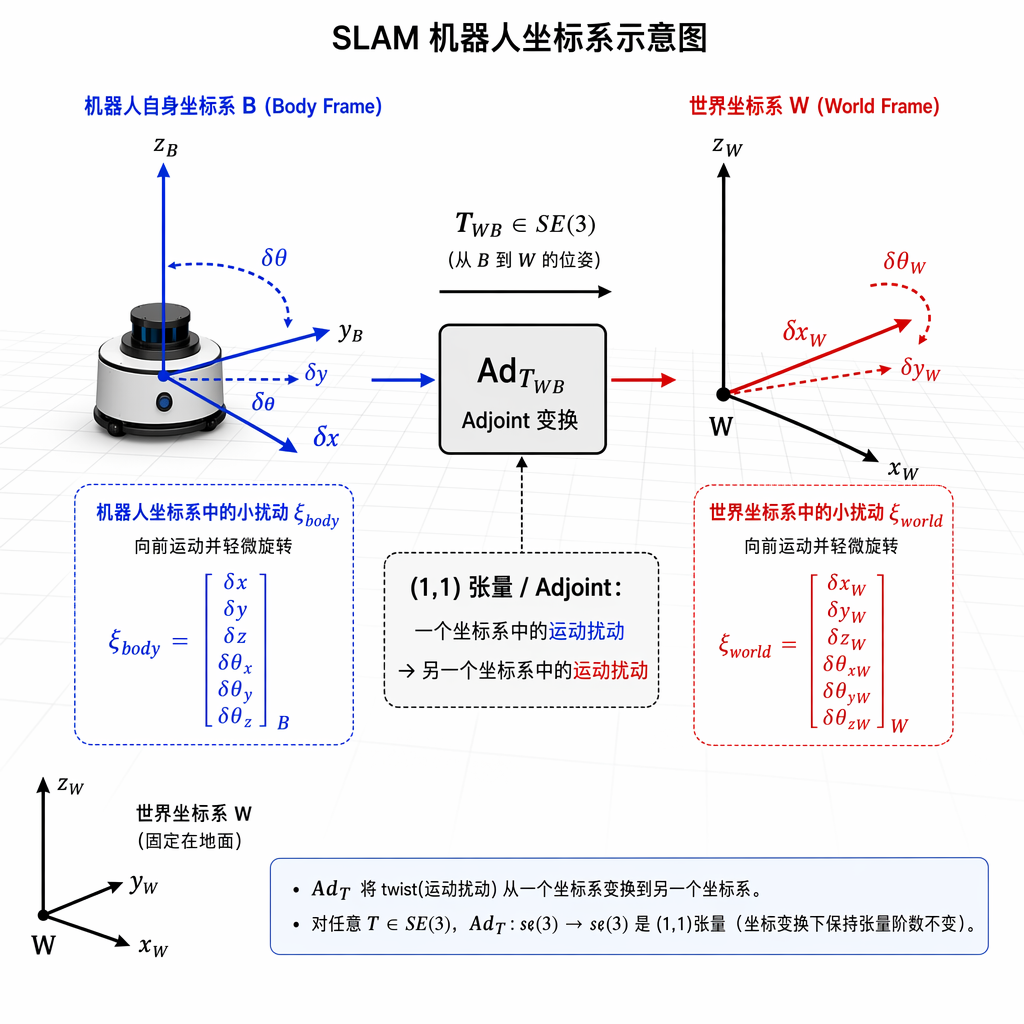
\includegraphics[width=0.74\textwidth]{assets/images/chapter4/4-3/1783529830604-907f3b1ba684.png}
    \captionof{figure}{伴随变换把不同坐标系中的局部扰动联系起来。}
    \label{fig:chapter4-adjoint}
\end{center}
\end{minipage}

\noindent\begin{minipage}{\textwidth}
\begin{slamcase}{李括号：$(1,2)$型}
李括号
\[
    [\cdot,\cdot]:\mathfrak g\times\mathfrak g\to\mathfrak g
\]
是两个局部运动输入、一个局部运动输出的双线性映射，属于$(1,2)$型结构。它刻画两种无穷小运动交换顺序产生的非交换修正，并在BCH公式和$\SE(3)$的旋转--平移耦合中出现。
\end{slamcase}

\begin{center}
    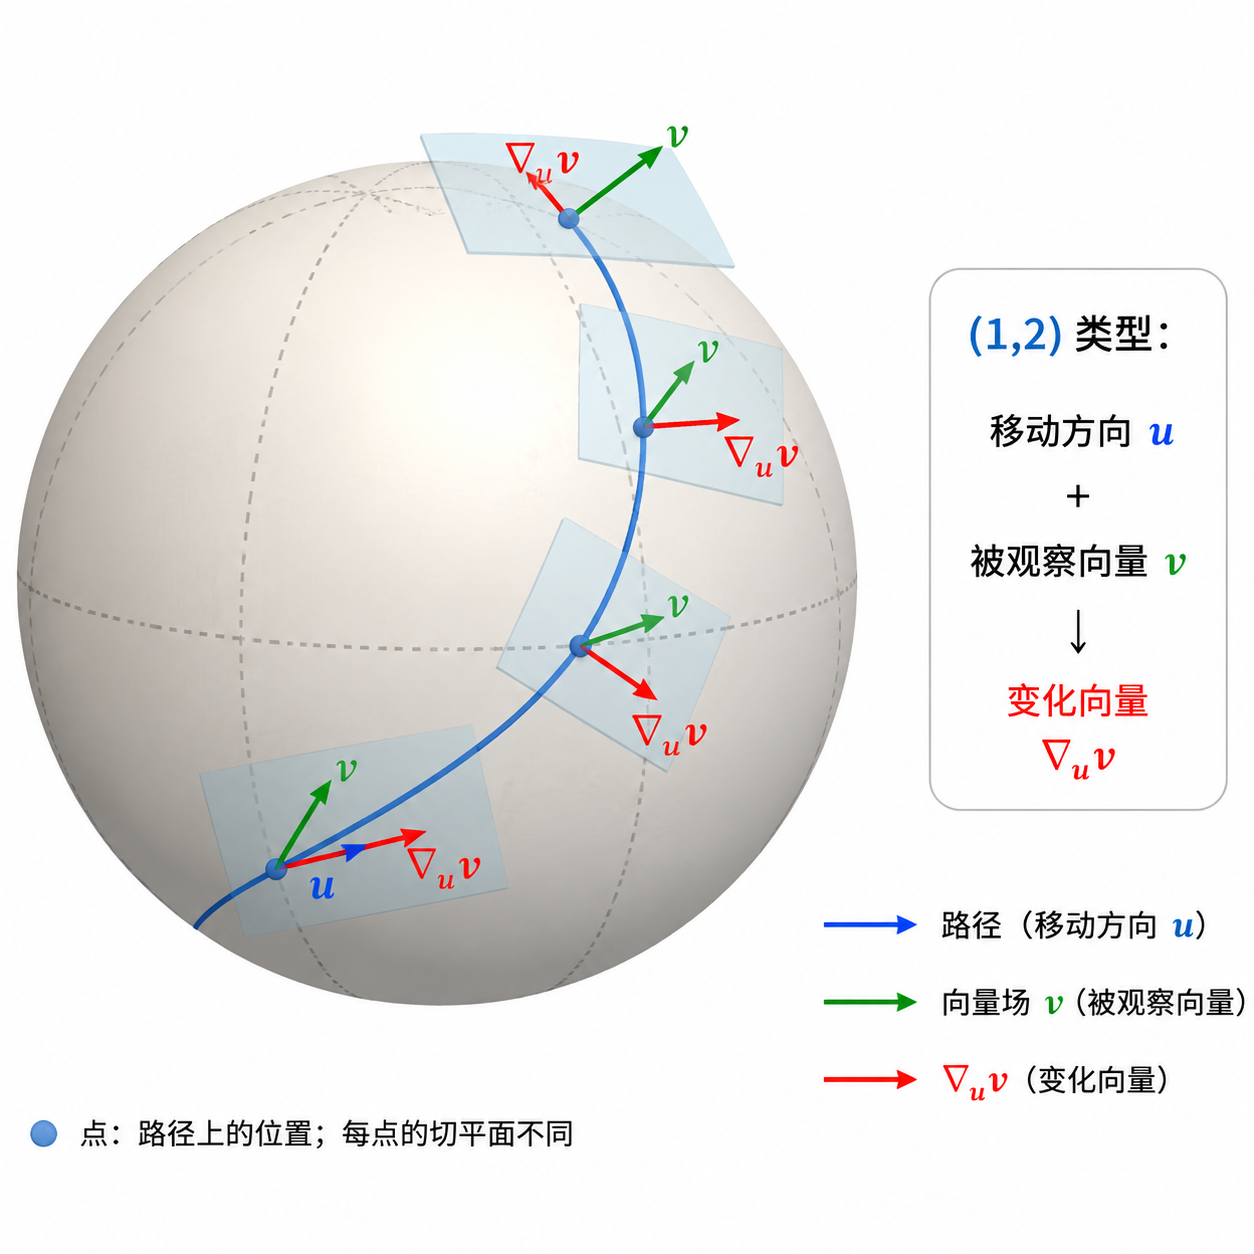
\includegraphics[width=0.74\textwidth]{assets/images/chapter4/4-3/1783528395477-b86af7104c3b.png}
    \captionof{figure}{两个局部方向通过双线性运算产生新的变化方向。}
    \label{fig:chapter4-bracket}
\end{center}
\end{minipage}

\noindent\begin{minipage}{\textwidth}
\begin{slamcase}{协方差与信息矩阵的类型}
若随机扰动$\delta x$被看作切空间$V$中的随机向量，则
\[
    \operatorname{Cov}(\delta x)=\mathbb E[\delta x\otimes\delta x]
\]
可视为$(2,0)$型对象；它描述向量扰动在各方向上的二阶扩散。另一方面，信息矩阵或Hessian近似自然作用为
\[
    H:V\times V\to\mathbb R,
\]
是$(0,2)$型双线性型。二者在选定基和内积后都表现为矩阵，但几何类型并不相同。
\end{slamcase}

\begin{center}
    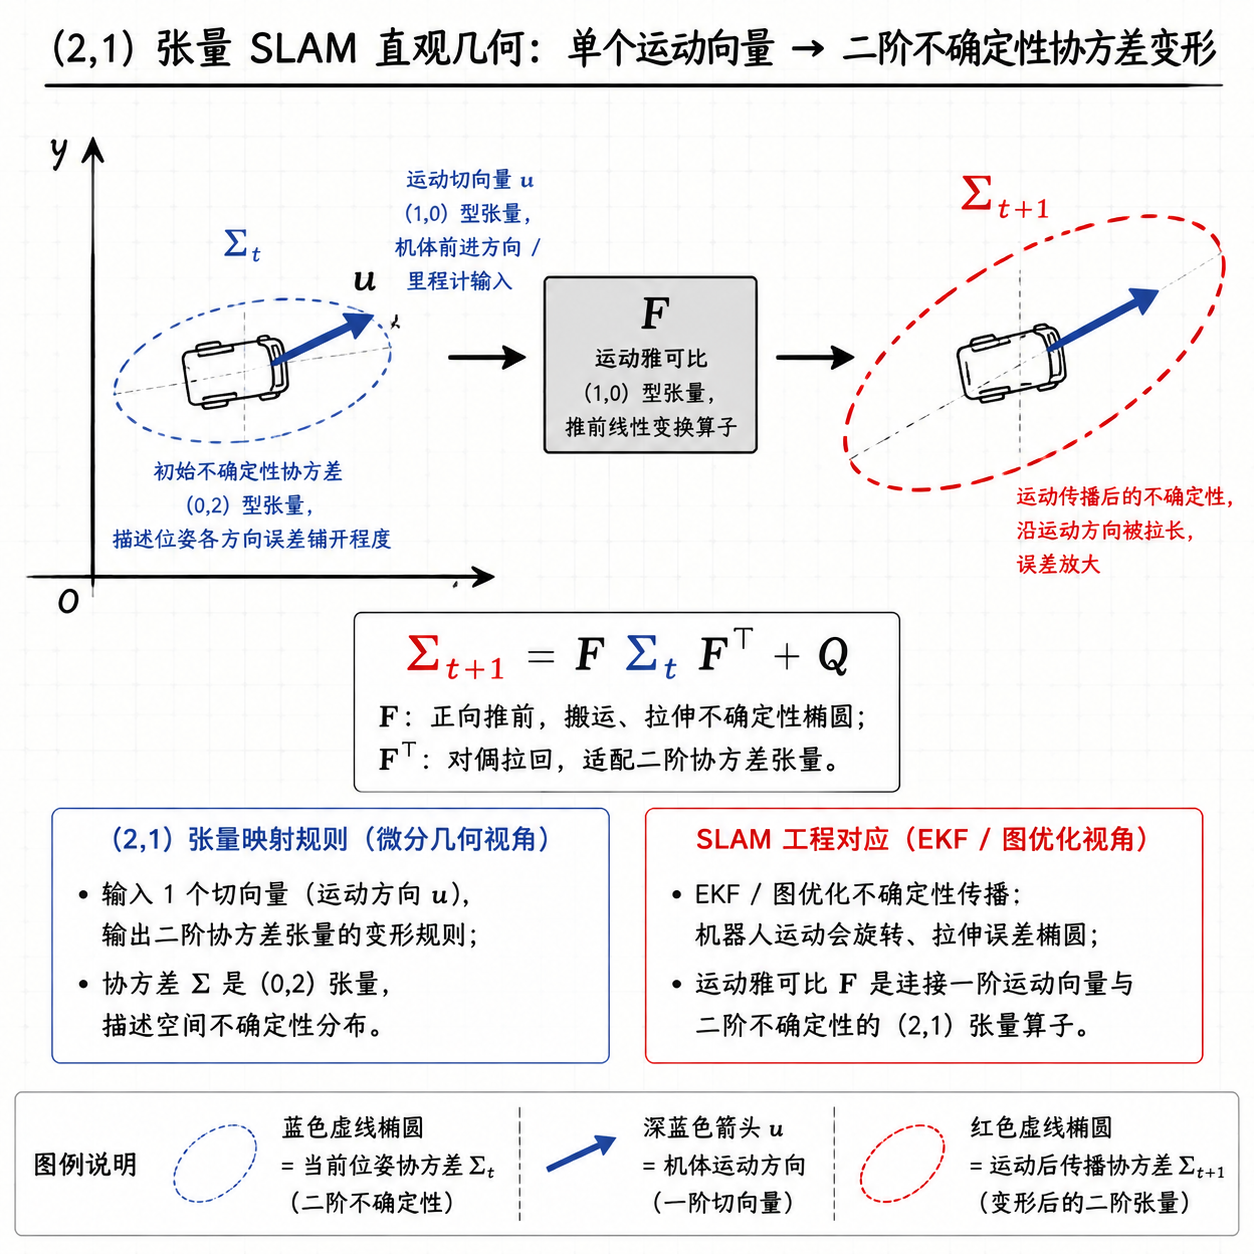
\includegraphics[width=0.74\textwidth]{assets/images/chapter4/4-3/1783535287928-22fb6aeeac5c.png}
    \captionof{figure}{局部扰动的二阶不确定性可以用协方差结构描述。}
    \label{fig:chapter4-covariance}
\end{center}
\end{minipage}

\noindent\begin{minipage}{\textwidth}
\begin{slamcase}{Jacobian拉回观测空间的二阶结构}
若$J:V\to W$是残差Jacobian，$W$上有观测信息双线性型$W_o$，则
\[
    H(u,v)=W_o(Ju,Jv)
\]
是状态扰动空间$V$上的$(0,2)$型双线性型。在矩阵坐标中，这正是
\[
    H=J^\top W_oJ.
\]
所以Gauss--Newton矩阵不是简单的矩阵乘法产物，而是观测空间二阶度量经Jacobian拉回状态空间后的表示。
\end{slamcase}

\begin{center}
    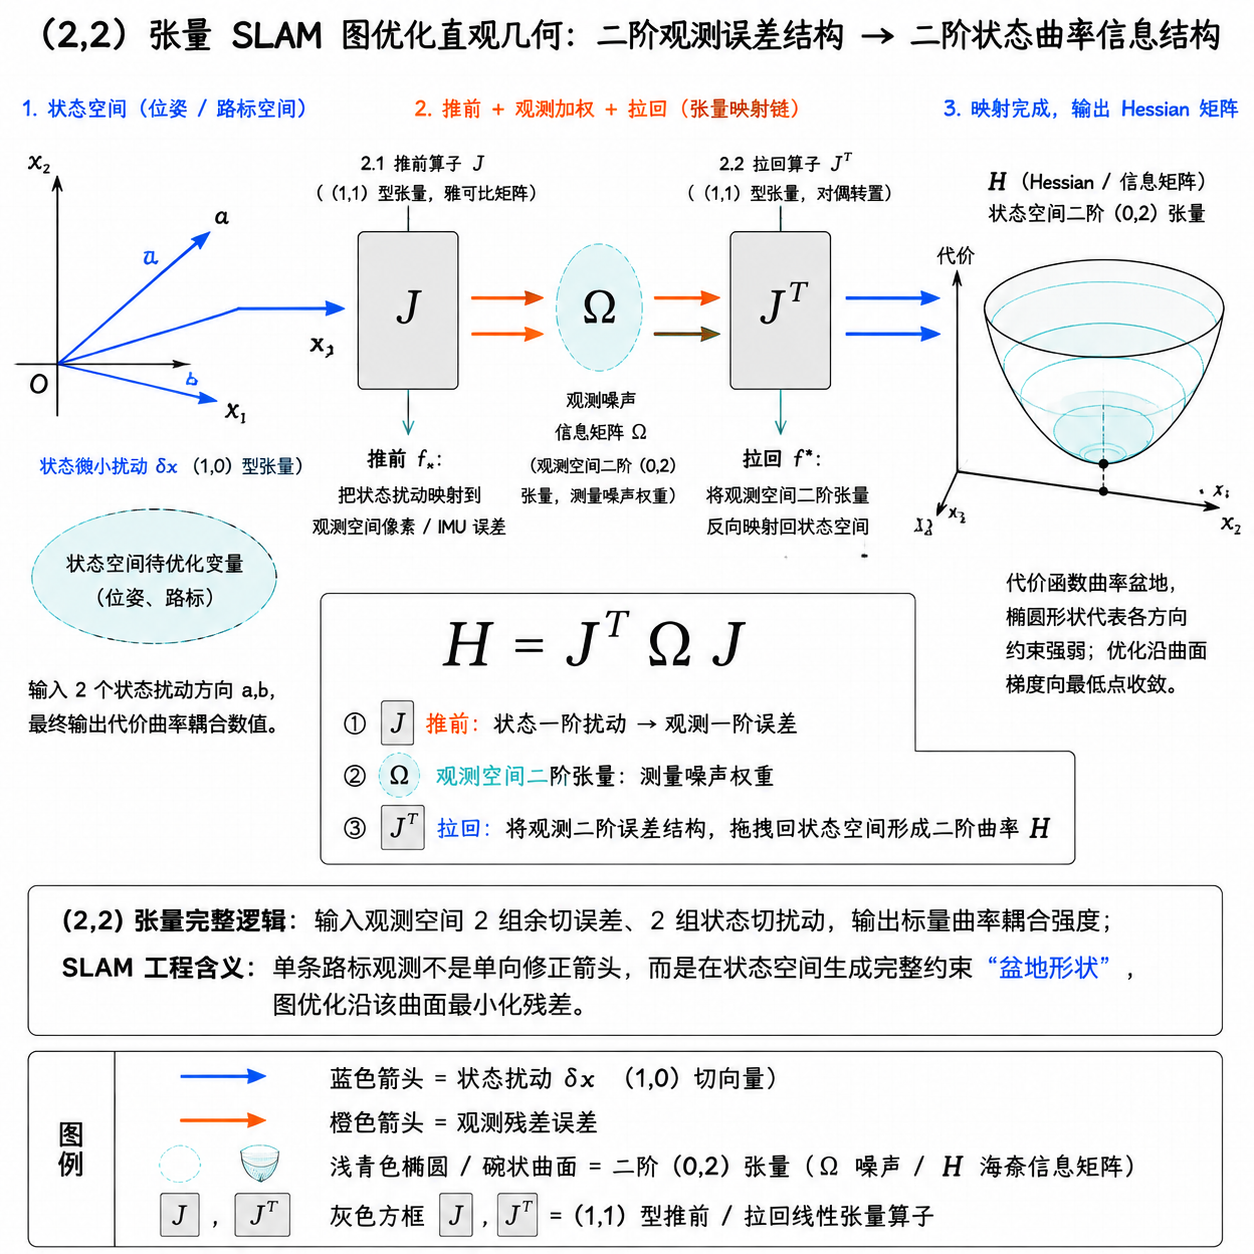
\includegraphics[width=0.74\textwidth]{assets/images/chapter4/4-3/1783535602448-f3a3cb307ac7.png}
    \captionof{figure}{观测空间中的二阶信息结构经Jacobian拉回到状态扰动空间。}
    \label{fig:chapter4-information-pullback}
\end{center}
\end{minipage}

%——————————————————————————————————%

\section{度量、长度与能量}

切空间提供局部线性结构，但仅有向量空间还不能比较不同方向的长度，也不能把协向量唯一地表示成向量。度量补充了内积、长度、角度和能量，并最终解释SLAM中梯度与加权最小二乘的几何含义。

\subsection{Riemann度量}

\begin{definition}[Riemann度量]
光滑流形$M$上的Riemann度量是对每个$p\in M$指定一个内积
\[
    \langle\cdot,\cdot\rangle_p:T_pM\times T_pM\to\mathbb R,
\]
满足正定性、对称性和双线性，并且对任意光滑向量场$X,Y$，函数$p\mapsto\langle X_p,Y_p\rangle_p$光滑。
\end{definition}

度量给出切向量的范数
\[
    \|v\|_p=\sqrt{\langle v,v\rangle_p}
\]
以及余切空间与切空间之间的音乐同构。对$f:M\to\mathbb R$，梯度由
\[
    df_p(v)=\langle\operatorname{grad}f(p),v\rangle_p,
    \qquad v\in T_pM
\]
定义。由此可见，$df_p$天然是协向量，而$\operatorname{grad}f(p)$是借助度量得到的切向量。

\subsection{曲线长度与能量}

设$\gamma:[a,b]\to M$为光滑曲线。其长度定义为
\[
    L(\gamma)=\int_a^b\|\dot\gamma(t)\|_{\gamma(t)}\,dt,
\]
能量定义为
\[
    E(\gamma)=\frac12\int_a^b\|\dot\gamma(t)\|_{\gamma(t)}^2\,dt.
\]
长度衡量曲线走过的总距离，能量衡量速度平方的累计。局部长度极小的曲线称为测地线；在有足够正则性的条件下，固定端点的测地线也是能量的临界曲线。

在欧氏空间中，所有点共享同一个切空间并使用同一个内积，因此长度和能量可直接写成普通向量积分。在一般流形上，$\dot\gamma(t)$属于随$t$变化的$T_{\gamma(t)}M$，度量正是把这些不同基点的局部速度逐点变成可比较的标量。

\subsection{从度量到SLAM代价}

残差空间$\mathbb R^m$通常使用标准内积，或使用噪声协方差诱导的加权内积
\[
    \langle u,v\rangle_W=u^\top Wv,
    \qquad W\succ0.
\]
于是多个观测的代价
\[
    F(x)=\frac12\sum_i r_i(x)^\top W_i r_i(x)
\]
可以理解为残差空间中的加权能量。对单个残差$r$，有
\[
    dF_x=(dr_x)^\ast(Wr(x)).
\]
若状态切空间在当前坐标中的度量矩阵为$G$，则
\[
    \operatorname{grad}F
    =G^{-1}J^\top Wr.
\]
当$G=I$时才简化为常见的$J^\top Wr$。因此，$J^\top Wr$在没有说明度量时首先应被理解为微分$dF_x$的坐标表示，而不是天然属于切空间的向量。

\subsection{局部二次模型与流形更新}

在当前状态$x$处，用局部切空间增量$\delta\xi$线性化残差：
\[
    r(x\boxplus\delta\xi)
    \simeq r(x)+J\delta\xi.
\]
Gauss--Newton在切空间中求解
\[
    \min_{\delta\xi}
    \frac12(r+J\delta\xi)^\top W(r+J\delta\xi).
\]
令局部二次模型的一阶导数为零，得到正规方程
\[
    J^\top WJ\,\delta\xi=-J^\top Wr.
\]
求解出的$\delta\xi$仍然是切空间坐标，不能直接把它与流形点相加；必须使用retraction返回流形：
\[
    x_{\mathrm{new}}=x\boxplus\delta\xi.
\]
对$\SE(3)$，第五章将选定右乘扰动并具体写成
\[
    T_{\mathrm{new}}=T\Exp(\delta\xi^\wedge).
\]
因此SLAM后端的统一结构是：在切空间中线性化和求解，在状态流形上更新，在残差空间中评价代价。

%——————————————————————————————————%

\section*{本章小结}

本章的主线可以压缩为以下几句话：
\begin{enumerate}
    \item 拓扑流形只提供局部欧氏性；兼容的$C^k$图册把坐标之间的微积分规则固定下来，形成可微流形。
    \item 光滑映射在局部坐标中表现为普通多元函数，微分同胚则表示两个空间在拓扑和可微结构上完全一致。
    \item $T_pM$由经过$p$的光滑曲线的瞬时速度组成，是局部线性化空间；$\SE(3)$的切空间有六个自由度，但$\SE(3)$本身不是$\mathbb R^6$。
    \item 推前把切向量送到输出空间，拉回把协向量送回输入空间；SLAM中的$J$和$J^\top r$分别来自这两个方向的线性映射。
    \item 沉浸是微分处处单射，嵌入还要求像集保持全局拓扑；这解释了八字曲线、四元数双覆盖以及$\SO(3)\hookrightarrow\mathbb R^9$之间的区别。
    \item 向量空间、对偶、张量和Riemann度量规定了“方向、测量、二阶结构和长度”这些对象的类型，避免把协向量、梯度和矩阵表示混为一谈。
    \item Gauss--Newton在切空间中求解增量，再通过retraction回到流形；这正是从微分几何走向李群位姿扰动的桥梁。
\end{enumerate}
